
\subsection{Cyclus Fuel Cycle Simulator}

\begin{frame}[ctb!]
  \frametitle{Cyclus Framework}
  \footnotesize{
  Cyder was designed for use within the Cyclus Fuel Cycle Simulator Framework.
  \begin{figure}[htb!]
    \begin{center}
      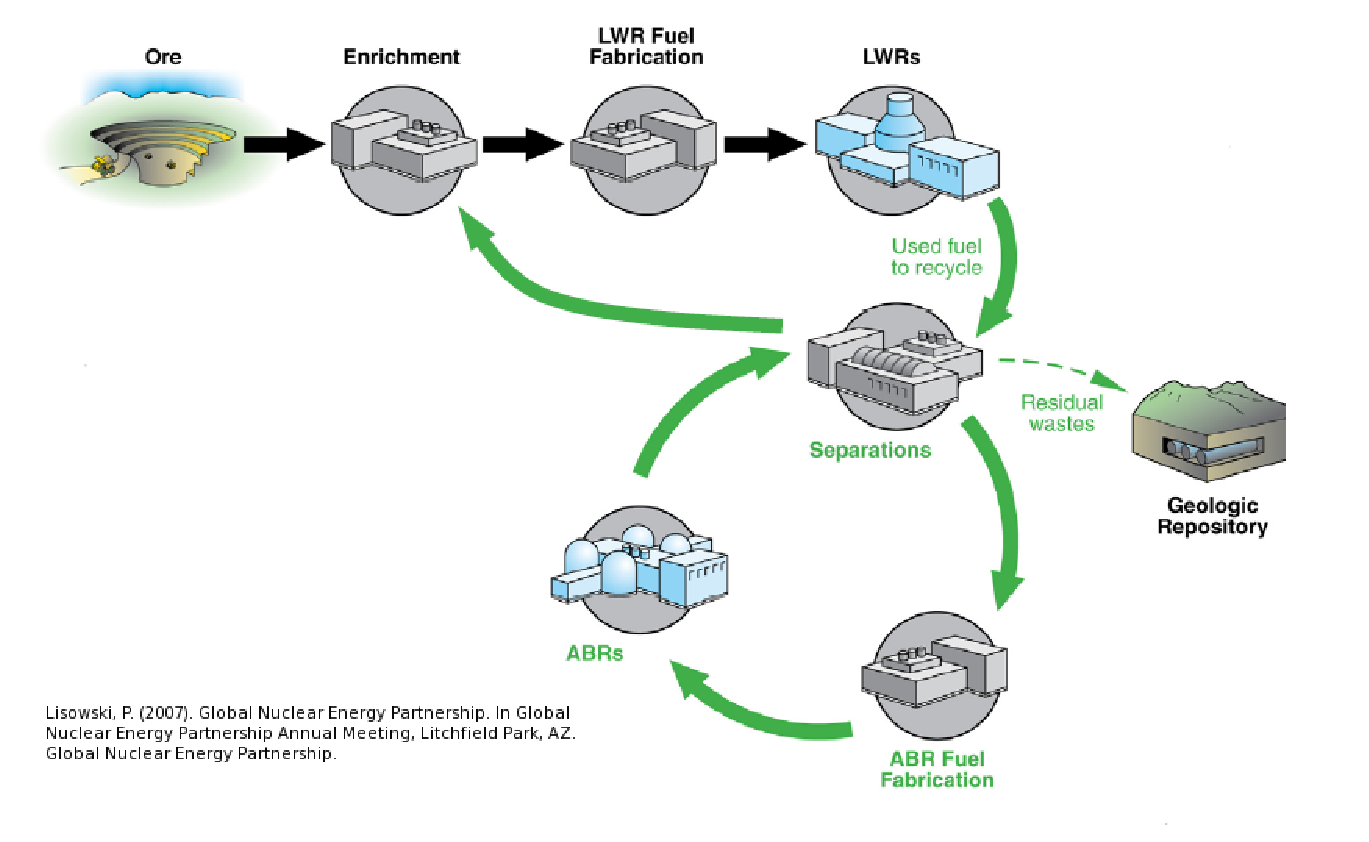
\includegraphics[width=0.6\textwidth]{./cyder/images/simulations.eps}
    \end{center}
    \caption{The Cyclus simulator framework provides an environment for fuel 
    cycle analysis.}
    \label{fig:simulations}
  \end{figure}
  %Cyclus Figure
  %Simulation Figure
}
\end{frame}

\subsection{Modular Barrier Components}

\begin{frame}[ctb!]
  \frametitle{Cyder Framework}
  \footnotesize{
The Cyder repository model architecture is intended to modularly permit 
exchange of disposal system Component models (e.g., detailed nuclide transport 
model vs. less detailed) and data (e.g., exchange clay for granite geologic 
data) and accept arbitrary waste stream isotopic compositions.  
  \begin{figure}[htbp!]
    \begin{center}
      \includegraphics[width=0.6\textwidth]{cyder/images/componentLoading.eps}
      \caption{The Cyder architecture modularly permits exchange of models and data.}
    \end{center}
  \end{figure}
}
\end{frame}

\begin{frame}[ctb!]
  \frametitle{Cyder Framework : Waste Stream Acceptance}
  \footnotesize{
  
To participate in fuel cycle simulation repository model must accept arbitrary 
spent fuel and high level waste streams. A waste stream is a material data 
object resulting from the Cyclus simulated fuel cycle.  
  \begin{figure}[htbp!]
    \begin{center}
      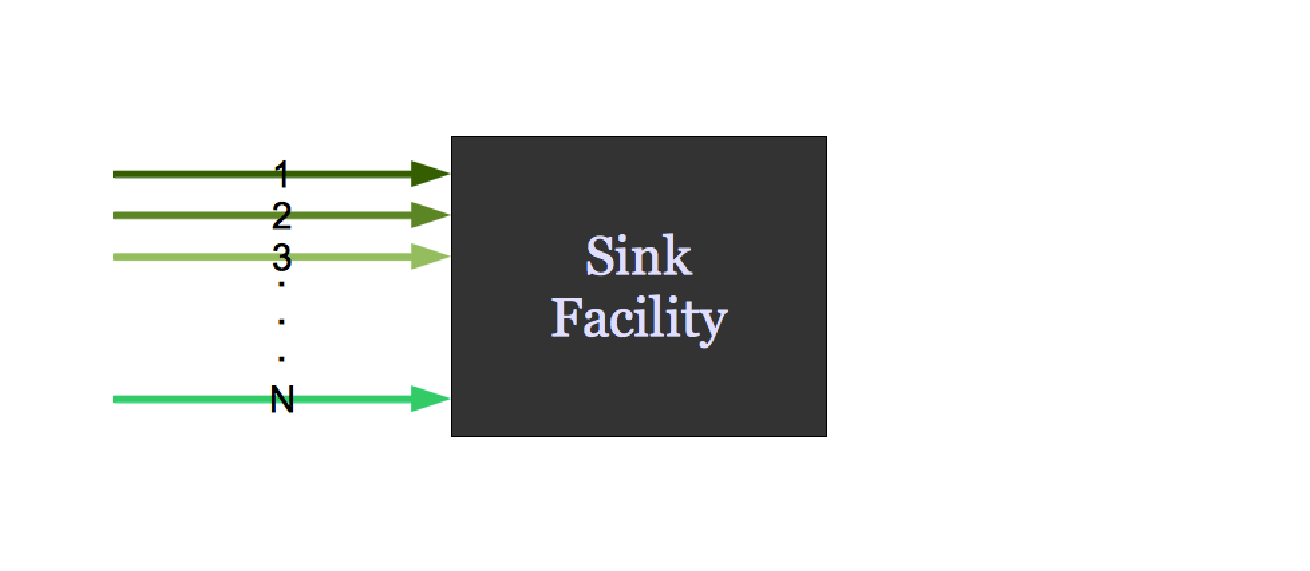
\includegraphics[height=5cm]{./cyder/images/sinkfacility.eps}
    \end{center}
    \caption{ The Cyder Facility dynamically accepts material from the 
    coupled fuel cycle simulation.} 
    \label{fig:sinkfacility}
  \end{figure}
% Sink Facility ?
}
\end{frame}

\begin{frame}[ctb!]
  \frametitle{Cyder Framework : Waste Stream Conditioning}
  \footnotesize{

    \textbf{Waste conditioning} is the process of packing a waste stream into an appropriate 
waste form.  The Cyder model loads discrete waste forms with discrete waste 
stream contaminant vectors as depicted in Figure \ref{fig:ws_conditioning}.
  
\begin{figure}[htbp!]
\begin{center}
\def\svgwidth{.5\textwidth}
\input{./cyder/images/ws_conditioning.eps_tex}
\end{center}
\caption{Waste streams are conditioned into the appropriate waste form 
according to user-specified pairings.}
\label{fig:ws_conditioning}
\end{figure}
}
\end{frame}

\begin{frame}[ctb!]
  \frametitle{Cyder Framework : Waste Form Packaging}
  \footnotesize{

    \textbf{Waste packaging} is the process of placing one or many waste forms into a 
containment package. Once the waste stream has been conditioned into a waste 
form, that waste form Component is loaded into a waste package Component as 
depicted in Figure \ref{fig:wf_packaging}.  

\begin{figure}[htbp!]
\begin{center}
\def\svgwidth{.5\textwidth}
\input{./cyder/images/wf_packaging.eps_tex}
\end{center}
\caption{Waste forms are loaded into the appropriate waste package 
according to user-specified pairings.}
\label{fig:wf_packaging}
\end{figure}
}
\end{frame}

\begin{frame}[ctb!]
  \frametitle{Cyder Framework : Waste Package Emplacement}
  \footnotesize{
  
\begin{columns}[c]
  \column{0.3\textwidth}
  Finally, the waste package is \textbf{emplaced} in a buffer component which 
contains many other waste packages spaced evenly in a grid as in Figure 
\ref{fig:repo_layout}. Repository depth, $\Delta z$, waste package spacing, 
$\Delta x$, and tunnel spacing, $\Delta y$ are user specified.

  \column{0.7\textwidth}

\begin{figure}[htbp!]
\begin{center}
\def\svgwidth{.5\textwidth}
\input{./cyder/images/repo_layout.eps_tex}
\end{center}
\caption{ The grid is defined by the user.  }
\label{fig:repo_layout}
\end{figure}
\end{columns}

}
\end{frame}

